\section{Vanilla}
\label{sec:vanilla}

\begin{spice}\label{spice:vanilla}
\textsc{Vanilla} \hfill \href{https://powo.science.kew.org/taxon/262578-2}{POWO} \\
\textbf{English:} \textit{vanilla}. 
\textbf{Arabic:} {\arabicfont{فانيليا}} \textit{fānīliyā}. 
\textbf{Chinese:} {\tradchinesefont{香草}} \textit{xiāngcǎo} [fragrant-herb]; Cantonese: 雲呢拿 \textit{wan4 nei1 laa4-2}. 
\textbf{Hungarian:} \textit{vanília}.  \\
\noindent{\color{black}\rule[0.5ex]{\linewidth}{.5pt}}
\begin{tabular}{@{}p{0.25\linewidth}@{}p{0.75\linewidth}@{}}
Plant species: & \taxonn{Vanilla planifolia}{Jacks. ex Andrews} (syn. \taxonn{V. fragrans}{Ames}); \textit{\taxonn{V. tahitensis}{J.W. Moore}; \taxonn{V. pompona}{Schiede}} \\
Family: & \textit{Orchidaceae} \\
Plant part used: & fruit \\
Region of origin: & Tropical America \\
Cultivated in: & Madagascar; Indonesia; Mexico; Papua New Guinea; China \\
Color: & dark brown pod; creamy white extract \\
\end{tabular}
\end{spice}

\begin{figure}[!ht]
	\vspace{-4ex}
	\centering
	\subfloat[]{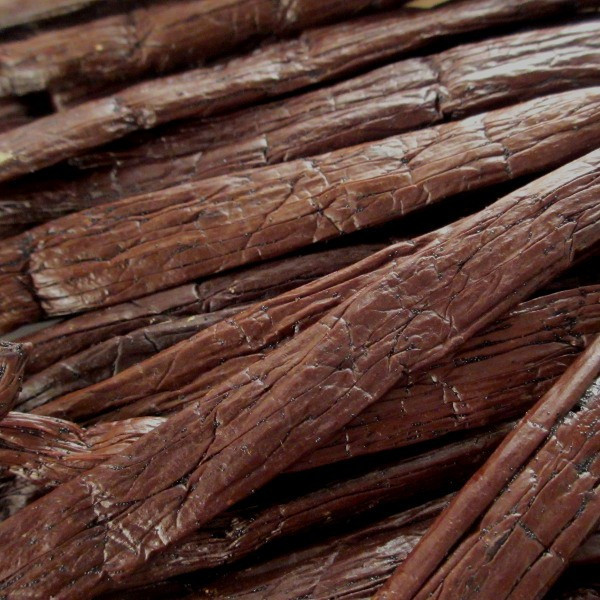
\includegraphics[width=0.3\linewidth]{imgs/spices/vanilla-1.jpg}}
	\hfill
	\subfloat[]{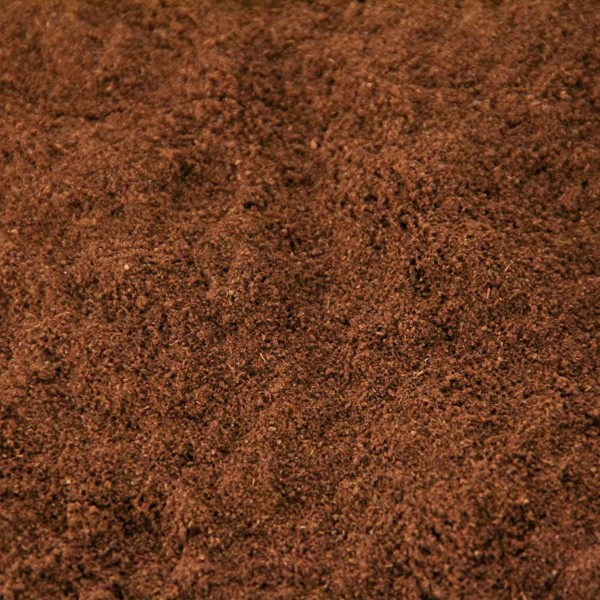
\includegraphics[width=0.3\linewidth]{imgs/spices/vanilla-2.jpg}}
	\hfill
	\subfloat[]{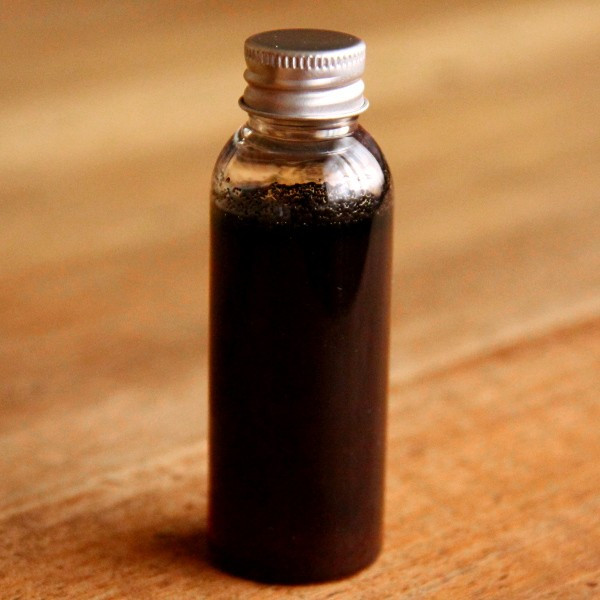
\includegraphics[width=0.3\linewidth]{imgs/spices/vanilla-3.jpg}}
	\caption{vanilla... \taxon{Vanilla planifolia?}. Credits: Aromatiques; Wikimedia Commons (CC4.0)}\footnote{\url{https://commons.wikimedia.org/wiki/File:Saffron_Flowers_in_Khorasan,_Iran.jpg}}
	\label{fig:vanilla_imgs}
\end{figure}




Vanilla ``beans'' are the elongated, dried and cured fruits of the plant \textit{Vanilla planifolia} and spp.\footnote{} with a well-known, attractive aroma. In its relatively recent career, vanilla (better said, vanilla extract) spread around the globe with intensity and haste, and it is an unavoidable flavouring and fragrance of the modern world. From ice cream to candles, baking and aromatherapy, vanilla was so overused commercially, that it became a synonym for 'plain and conventional'. Because its labour intensive production, vanilla is still the second most expensive spice today after saffron??.

\subsection{The Botany, Origin, and Cultivation of Vanilla }

The vanilla vine is an epiphytic\footnote{A plant that grows on other plants.} orchid,  with fleshy leaves and yellowish flowers \parencite[282]{van_wyk_culinary_2014}. 
The fruits, often called ``beans'' or ``pods'' are long and thin, and contain thousands of seeds. It is indigenous to tropical America. There are three species of vanilla that are widely cultivated, all  originally from Mesoamerica. \textit{V. planifolia} is grown on various islands of the Indian Ocean, mainly Madagascar, Réunion, Comoros, and the Seychelles. \textit{V. tahitensis} is found on the South Pacific (it escaped cultivation on the Society islands and now grows on trees), while \textit{V. pompona} is the species of Central and South America and the West Indies. More than two thirds of the world's vanilla comes from Madagascar and Indonesia (FAOSTAT).

Plants are grown from cuttings, and require moist, tropical conditions. Until the \nth{19} century, Mexico enjoyed a monopoly on vanilla production, which was broken by the French, who transplanted it to their colonies of Réunion and Madagascar on the Indian Ocean, and later the Dutch to Java \parencite[282]{van_wyk_culinary_2014}.
This was made possible by a 12-year-old slave boy, Edmond Albius, pioneered a technique on the island of Réunion to hand-pollinate the plants in 1841, a feat that was almost stolen from him by a famous French botanist. Pollination is absolutely necessary (a task naturally performed by hummingbirds and bumblebees), which makes it the world's only hand-pollinated crop \parencite[959]{mabberley_mabberleys_2017}, and drives the price high. The seed-pods are hand picked when near-ripe and still green. Vanilla production requires a rigorous treatment: the beans are briefly put in boiling water, whence the heat disrupts the maturing process and activates enzymes responsible for vanillin production -- the main compound that supplies the flavour. Then, the beans are dried on the sun for weeks, during which the vanilla sticks attain their dark brown, shiny colour. In some cases the vanilla beans are left in boxes to ferment up to 9 months, to attain quality flavour \parencite[282]{van_wyk_culinary_2014}. This often results in an effect where the tiny, white vanillin crystals are noticeable on the beans, similar to frost.



%Chemistry


% Flavour compounDs The major flavour compound is vanillin (4-hydroxy-3-methoxybenzaldehyde), present in the cured fruits at a level of about 3\%.4,5 The green fruits contain vanillin-glycoside as a nonvolatile flavour precursor, which is enzymatically hydrolysed to glucose and vanillin during the curing process, so that the vanillin becomes visible as small white crystals on the surface of cured fruits. There are numerous minor compounds, including vanillic acid, 4-hydroxybenzaldehyde, 4-hydroxybenzoic acid and vanilla vitispirane, all contributing to some extent to the flavour and aroma.4,5 Synthetic vanillin, produced through semi-synthesis from eugenol (or wood pulp), is a cheap substitute for real vanillin because it lacks the chemical complexity of the natural product. notes Vanillin and related compounds occur in other natural products, such as African white ginger (powdered tubers of Mondia whitei) and most famously, oak-aged wine. Seeds of the tonka bean (Dipteryx odorata) have a spicy aroma similar to vanilla and almonds and have become an alternative to vanilla for flavouring ice cream, custard and other milk-based desserts.

% MABBERLEY
% V. planifolia Andrews ('V. mexicana', trop. Am.) – first Am. orchid figured in Eur. (Codex Badianus, 1552) used by Aztecs to flavour cocoa, cult. for orn. & for long fr. (berry; 'pod', without vanillin when unripe (6\% when mature), vanilloside breaking down to v. & glucose on ripening over 9 months), when cured source of v. extract (esp. in Madag. where anther & stigma have to be pressed together as poll. euglossine bee absent (world’s only hand-poll. crop) – pioneered 1841 by 12-yr-old slave from Réunion; all W I Ocean stock allegedly from a single cutting in Jardin des Plantes, Paris, coll. Veracruz)), although vanillin synth. from eugenol from cloves in 1891, pods still used in cooking by the discriminating & worth \$60–80 M a yr, (Madag. alone 3 K t a yr by 2005), but most flavouring today ('vanilla essence') is from wood pulp as a byproduct of paper-making & from coal-tar (toluene); V. × tahitensis J.W. Moore (V. p . × V. odorata C. Presl (trop. Am.), Tahiti vanilla,) also imp., esp. Pacific is.


% %USES
% culinary uses Whole fruits are an expensive but important flavourant for chocolate, ice cream, custards, milkshakes, puddings, various sweet dishes, confectionery, sweets, sugar, preserved fruits, soft drinks and liqueurs.3 The whole vanilla bean can be added to the dish and removed again for future use. It is often split lengthwise and the soft, aromatic pulp scraped out. The presence of minute black seeds in a homemade ice cream is therefore a sign of quality and authenticity. 

\subsection{The History of Vanilla}

The Aztecs, but originally Mexicans of Vera Cruz, used vanilla (tlilxochitl) to flavour cacao drinks.1,2 A Mexican monopoly was broken when plantations were established on Réunion and Madagascar by the French and on Java by the Dutch.1,2 Today, vanilla is also cultivated in other tropical regions, including the West Indies, Central America and Indonesia. 







% Pronunciation:
%  Brit. Hear pronunciation/vəˈnɪlə/
% , United States Hear pronunciation/vəˈnɪlə/
% Forms:  Also 1600s vaynilla. β. 1600s vinello-, 1700s vanello, 1700s–1800s vanelloe (1700s vaneloe); 1700s vanilio, vanillio, 1700s–1800s vanillo.(Show Less)
% Frequency (in current use):  Show frequency band information
% Etymology: In earlier use < older Spanish vaynilla , now vainilla , diminutive of vaina ( < Latin vāgīna vagina n.) sheath. Subsequently < modern botanical Latin Vanilla , from the same source. Compare Italian vainiglia , Portuguese bainilha , baunilha , French vanille vanille n.(Show Less)

% The majority of the world's vanilla is the V. planifolia species, more commonly known as Bourbon vanilla (after the former name of Réunion, Île Bourbon) or Madagascar vanilla, which is produced in Madagascar and neighboring islands in the southwestern Indian Ocean, and in Indonesia. Madagascar's and Indonesia's cultivations produce two-thirds of the world's supply of vanilla.




\subsection{The Names of Vanilla}
\label{sec:names_of_vanilla}

\subsubsection{English}

% ``for weak phlegmatique, and windy stomachs, they added \textit{Xochinacaztli}, or your Orichelas\footnote{\textit{Cymbopetalum penduliflorum}}''

The English word \textit{vanilla} was loaned from Spanish \textit{vainilla} and attested first in 1662: ``[...] so they added \textit{Tlilxochitl}, or the \textit{Vaynillas} [to the chocolate] for the like ends, and to strengthen the brain, and womb.'' \parencite[11]{stubbe_indian_1662}. The author here is explaining how the ``Indians'' -- the Aztecs -- flavoured their chocolate drinks. Spanish `vainilla', used for the American aromatic plant,  was first recorded in 1555.\textit{Vainilla}, literally `little vegetable pod', is the diminutive form of \textit{vaina}, meaning `scabbard, sheath' or `shell, husk' in the botanical sense.  \parencites[596]{corominas_breve_1987}[538]{gomez_de_silva_elseviers_1985}. \textit{Vaina} descended from Latin \textit{vāgīna} `scabbard, sheath; covering, holder of anything', i.e. husks that enclose an ear of grain 
% \LS{vāgīna}. 


\begin{etymology}\label{ety:vanilla}
English \textit{vanilla }, 1662
< Spanish \textit{vainilla} `id.' [little sheath, little pod], from \textit{vaina/vaína} `scabbard, sheath; pod, husk' + \textit{-illa} diminutive suffix, 1555
< Latin \textit{vāgīna} `scabbard, sheath; covering, holder of anything', esp. husks that enclose an ear of grain; also by anatomical figurative sense, origin of vagina\footnote{\textcite[vanilla]{oed}; \textcites[538]{gomez_de_silva_elseviers_1985}[596]{corominas_breve_1987}; \textcite[vāgīna]{lewis_latin_1879}}
\end{etymology}

% \begin{etymology}\label{ety:vanilla}
% English \textit{vanilla }
% < Spanish \textit{vainilla} `id.' [little sheath, little pod] (\textit{vaina} `sheath; pod' + \textit{-illa} diminutive)
% < Spanish \textit{vaina} `scabbard, sheath; pod, husk'
% < Latin \textit{vāgīna} `scabbard, sheath; covering, holder of anything'
% \footnote{OED; Gómez de Silva, 1985 p. 538; Corominas, 1987 p. 596}\end{etymology}


\begin{table}[!ht]
\centering
\begin{tabularx}{\textwidth}{@{}l>{\itshape \small}lL>{\small}l@{}}
\toprule
\textbf{\#} & \multicolumn{1}{l}{\textbf{Species}} & \multicolumn{1}{l}{\textbf{Name}} & \multicolumn{1}{l}{\textbf{Source}} \\
\midrule
1	& Vanilla planifolia	& Bourbon vanilla	& \textcite{wikipedia} \\
2	& Vanilla planifolia	& French vanilla	& \textcite{wikipedia} \\
\textbf{3}	& \textbf{Vanilla spp.}	& \textbf{vanilla}	& \textbf{\textcite{van_wyk_culinary_2014}} \\
4	& Vanilla tahitensis	& Tahitian vanilla	& \textcite{wikipedia} \\
\bottomrule
\end{tabularx}
\caption{Various names for vanilla in English.}
\label{table:names_vanilla_en}
\end{table}



\subsubsection{Arabic}

\begin{table}[!ht]
\centering
\begin{tabularx}{\textwidth}{@{}l>{\itshape \small}lr>{\itshape}lL>{\small}l@{}}
\toprule
\textbf{\#} & \multicolumn{1}{l}{\textbf{Species}} & \multicolumn{1}{l}{\textbf{Name}} & \multicolumn{1}{l}{\textbf{Tr.}} & \multicolumn{1}{l}{\textbf{Gloss}} & \multicolumn{1}{l}{\textbf{Source}} \\
\midrule
\textbf{1}	& \textbf{Vanilla planifolia}	& \textbf{فانيليا}	& \textbf{fānīliyā}	& \textbf{phonetic}	& \textbf{\textcite{baalbaki_-mawrid_1995}} \\
2	& Vanilla planifolia	& ونيلية	& wanīliyya	& 	& \textcite{baalbaki_-mawrid_1995} \\
\bottomrule
\end{tabularx}
\caption{Various names for vanilla in Arabic.}
\label{table:names_vanilla_ar}
\end{table}



\subsubsection{Chinese}

\begin{table}[!ht]
\centering
\begin{tabularx}{\textwidth}{@{}l>{\itshape \small}ll>{\itshape}lL>{\small}l@{}}
\toprule
\textbf{\#} & \multicolumn{1}{l}{\textbf{Species}} & \multicolumn{1}{l}{\textbf{Name}} & \multicolumn{1}{l}{\textbf{Tr.}} & \multicolumn{1}{l}{\textbf{Gloss}} & \multicolumn{1}{l}{\textbf{Source}} \\
\midrule
\textbf{1}	& \textbf{Vanilla planifolia}	& \textbf{\tradchinesefont{香草}}	& \textbf{xiāngcǎo}	& \textbf{fragrant-grass/herb}	& \textbf{\textcite{defrancis_abc_2003}} \\
\bottomrule
\end{tabularx}
\caption{Various names for vanilla in Chinese.}
\label{table:names_vanilla_zh}
\end{table}



\subsubsection{Summary}

\begin{table}[!ht]
    \caption{Conventionalized names for vanilla in English, Arabic, and Chinese, found in dictionaries.}
\centering
\begin{tabularx}{\textwidth}{@{}ll>{\itshape}lLl>{\small}l@{}}
\toprule
\textbf{\#} & \textbf{Language} & \multicolumn{1}{l}{\textbf{Term}} & \textbf{Gloss} & \textbf{Loan} & \multicolumn{1}{l}{\textbf{Source}} \\
\midrule
1	& English	& vanilla	& 	& yes	& \textcite{oed} \\
\midrule
1	& Arabic	& fānīliyā	& 	& yes	& \textcite{baalbaki_-mawrid_1995} \\
2	& Arabic	& wanīliyya	& 	& yes	& \textcite{baalbaki_-mawrid_1995} \\
\midrule
1	& Chinese	& xiāngcǎo	& fragrant-grass/herb	& no	& \textcite{defrancis_abc_2003} \\
\bottomrule
\end{tabularx}
\label{table:names_vanilla}
\end{table}















% OED

% Etymology: In earlier use < older Spanish vaynilla , now vainilla , diminutive of vaina ( < Latin vāgīna vagina n.) sheath. Subsequently < modern botanical Latin Vanilla , from the same source. Compare Italian vainiglia , Portuguese bainilha , baunilha , French vanille


% English,vanilla
% Spanish,vainilla
% Latin,vāgīna

% EE:
% vanilla 

% (pod of) climbing orchid of the genus Vanilla XVII; aromatic substance obtained therefrom XVIII. — Sp. vainilla, dim. of vaina sheath:- L. vāgīna VAGINA.

% OE:
% vanilla (n.)

% 1660s, "pod of the vanilla plant," from Spanish vainilla "vanilla plant," literally "little pod," diminutive of vaina "sheath," from Latin vagina "sheath of an ear of grain, hull of a plant" (see vagina). So called from the shape of the pods. European discovery 1521 by Hernando Cortes' soldiers on reconnaissance in southeastern Mexico. Meaning "flavoring extracted from the vanilla bean" is attested by 1728.

% Adjectival meaning "conventional, of ordinary sexual preferences" is by 1970s, probably from the notion of whiteness and the common choice of vanilla ice cream; vanilla as figurative of a plain and conventional choice (without reference to sex) seems to date to the late 19c. as a noun, by 1940s (often plain vanilla) as an adjective.

% MW:
% in sense 1a, from New Latin, from Spanish vainilla vanilla; in other senses from Spanish vainilla pod, vanilla, diminutive of vaina sheath, from Latin vagina — more at vagina

% First Known Use: 1662 (sense 2a)

% borrowed from New Latin, going back to Latin vāgīna “scabbard, sheath,” of uncertain origin
% Note: Latin vāgīna as an anatomical term does not appear to be earlier than the 16th century, though Roman use of the word as a sexual metaphor is as old as Plautus’s comedy Pseudolus (“ … quom tu ibas simul, conveniebatne in vaginam tuum machaera militis?” - “ … when you were going with him, did the soldier’s sword fit in your scabbard?”). Latin vāgīna has been compared with Lithuanian vóžti “to close with a lid or cover, shut” (from Indo-European *u̯eh2ǵ-?), though a link is doubtful given the vague sense connection and lack of other comparanda. According to Ernout and Meillet (Dictionnaire étymologique de la langue latine: histoire des mots, fourth edition, 1959), “undoubtedly a borrowed technical term” (“terme technique sans doute emprunté”).

% First Known Use: 1653 (sense 1a)


% AH:
% [Spanish vainilla, from Old Spanish, pod, from diminutive of vaina, sheath, from Latin vāgīna.] 

% WK:
% Borrowed from Spanish vainilla, a diminutive form of vaina (“pod”). 